\begin{frame}{Why tensor networks?}

 \begin{columns}
        \begin{column}{.5\textwidth}
        \bi
        \only<1>{
        \item Hilbert space is {\Large big}}
        \only<2->{
        \item Hilbert space is {\Large too big}}
        \bi
        \item<2-> $\text{Dim} \left( \bigotimes\limits_{i=1}^{N} \mathcal{H}_i \right)= 2^N$
        \item <3-> Generic states are maximally entangled
        \ei
        \item <4-> Ground states of many-body systems are special
        \bi
        \item <5-> Tensor networks target area law states 
        \ei
        \ei
        \end{column}
        \begin{column}{.5\textwidth}%\raggedleft
            \only<2-3>{
            \begin{figure}[t]
                %%!TEX root = ../thesis.tex

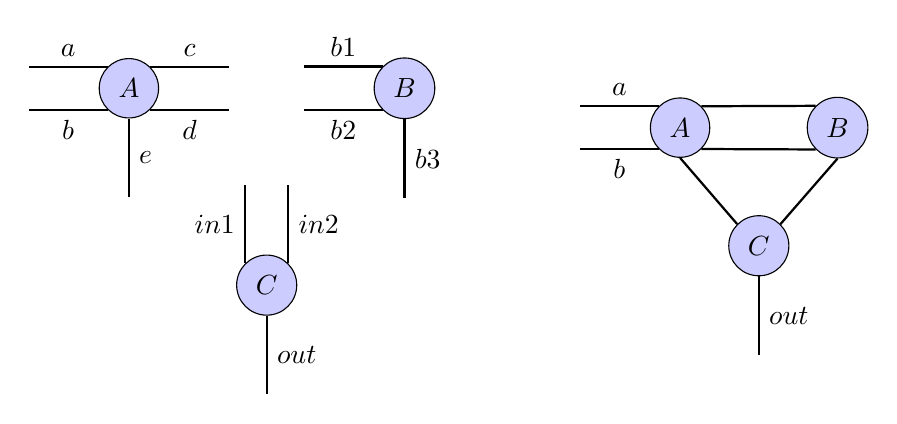
\begin{tikzpicture}

\node[det] (A) at (0,0) {$A$};
\draw[thick] (A.north east) -- node[above] {$c$} +(1,0);
\draw[thick] (A.south east) -- node[below] {$d$} +(1,0);
\draw[thick] (A.north west) -- node[above] {$a$} +(-1,0);
\draw[thick] (A.south west) -- node[below] {$b$} +(-1,0);
\draw[thick] (A.south) -- node[right] {$e$} +(0,-1);

\node[det] (B) at (3.5,0) {$B$};
\draw[thick] (B.north west) -- node[above] {$b1$} +(-1,0);
\draw[thick] (B.south west) -- node[below] {$b2$} +(-1,0);
\draw[thick] (B.south) -- node[right] {$b3$} +(0,-1);

\node[det] (C) at (1.75,-2.5) {$C$};
\draw[thick] (C.north west) -- node[left] {$in1$} +(0,1);
\draw[thick] (C.north east) -- node[right] {$in2$} +(0,1);
\draw[thick] (C.south) -- node[right] {$out$} +(0,-1);


\node[det] (Ap) at (7,-0.5) {$A$};
\node[det] (Bp) at (9,-0.5) {$B$};
\node[det] (Cp) at (8,-2) {$C$};

\draw[thick] (Ap.north east) -- (Bp.north west);
\draw[thick] (Ap.south east) -- (Bp.south west);
\draw[thick] (Ap.south) -- (Cp.north west);
\draw[thick] (Bp.south) -- (Cp.north east);

\draw[thick] (Ap.north west) -- node[above] {$a$} +(-1,0);
\draw[thick] (Ap.south west) -- node[below] {$b$} +(-1,0);
\draw[thick] (Cp.south) -- node[right] {$out$} +(0,-1);

\end{tikzpicture}

                %!TEX root = ../thesis.tex

%\beginpgfgraphicnamed{diagrams}
\begin{tikzpicture}[node distance=0.4cm]
%\tikzset{ellip/.style={ellipse (3 and 1), fill=blue!20, draw=black, inner sep=4pt}}
\tikzset{det/.style={circle=2pt,fill=blue!20,draw=black,inner sep=4pt}}
%\draw (1,1) ellipse [x radius=1cm,y radius=.5cm];
\node[ellipse, rotate=0, draw, fill=blue!20] (t) at (0,0) {\, \, $\psi$ \, \,};
\node (t1) at (-1.6, 0.6) {$i_1$};
\node (t2) at (-1.2 ,0.85) {$i_2$};
\node (t3) at (-0.8,1.1) {$i_3$};
\node (t4) at (-0.3,1.2) {$i_4$};
\node (t5) at (0.3, 1.2) {$i_5$};
\node (tN) at (1.6, 0.6) {$i_N$};
\node[rotate=-20] (d) at (0.6, 0.6) {...};
%\node (tl) at (1,-0.4) {$l$};
\draw[thick] (t1) -- (t);
\draw[thick] (t2) -- (t);
\draw[thick] (t3) -- (t);
\draw[thick] (t4) -- (t);
\draw[thick] (t5) -- (t);

\draw[thick] (tN) -- (t);
%\node[in of=t] {$\psi$};
\node (p) at (0,-1) {$|\psi \rangle = \sum \psi_{i_1 i_2 ... i_N} \vert i_1 i_2 ... i_N \rangle$};


%\draw  (-0.8,2.4) node (v1) {} ellipse (1.2 and 0.4);
%\draw  (v1) ellipse (0 and 0);
\end{tikzpicture}
%\endpgfgraphicnamed
            \end{figure}}
            \only<4-5>{
            \begin{figure}[htbp]
               \scalebox{0.6}{ %\beginpgfgraphicnamed{2d_area_law}

\begin{tikzpicture}

\foreach \i in {1,...,6}
\foreach \j in {1,...,6}
{ {
	%\node (G\i_\j) at (\j,\i) [spin] {\i..\j};
	\node (G\i_\j) at (\j,\i) [spin,inner sep=2pt,outer sep=3pt] {};
} }

\begin{pgfonlayer}{background}
\filldraw[fill=blue!20,rounded corners] (G1_1.south west) + (0,0) -- (G6_1.north west) -- (G6_3.north east) -- (G1_3.south east) -- cycle;
\filldraw[fill=blue!20,rounded corners] (G1_4.south west) + (0,0) -- (G6_4.north west) -- (G6_6.north east) -- (G1_6.south east) -- cycle;
\end{pgfonlayer}

\draw[thick,<->] (1,0.5) -- (6,0.5);
\node at (3.5,0.1) {$W$};
\draw[thick,<->] (0.5,1) -- (0.5,6);
\node at (0.1,3.5) {$L$};

\foreach \i in {1,...,6}
{
	\draw[very thick] (G\i_4) -- (G\i_3);
}

\end{tikzpicture}
%\endpgfgraphicnamed
%\begin{tikzpicture}

%\foreach \i in {1,...,6}
%\foreach \j in {1,...,6}
%{ {
%	%\node (G\i_\j) at (\j,\i) [spin] {\i..\j};
%	\node (G\i_\j) at (\j,\i) [spin,inner sep=2pt,outer sep=3pt] {};
%} }

%\begin{pgfonlayer}{background}
%\filldraw[fill=blue!20,rounded corners] (G1_1.south west) + (0,0) -- (G6_1.north west) -- (G6_3.north east) -- (G1_3.south east) -- cycle;
%\filldraw[fill=blue!20,rounded corners] (G1_4.south west) + (0,0) -- (G6_4.north west) -- (G6_6.north east) -- (G1_6.south east) -- cycle;

%\foreach \i in {1,...,6}
%\foreach \j / \k in {1/2,2/3,3/4,4/5,5/6}
%{ {
%	\draw[thick] (G\j_\i.center) -- (G\k_\i.center);
%} }

%\draw[thick] (G1_6.center) -- (G1_5.center);
%\draw[thick] (G1_4.center) -- (G1_3.center);
%\draw[thick] (G1_2.center) -- (G1_1.center);
%\draw[thick] (G6_5.center) -- (G6_4.center);
%\draw[thick] (G6_3.center) -- (G6_2.center);

%\end{pgfonlayer}

%\end{tikzpicture}

%\vspace{0.2in}

%\begin{tikzpicture}

%\foreach \i in {1,...,6}
%\foreach \j in {1,...,6}
%{ {
%	%\node (G\i_\j) at (\j,\i) [spin] {\i..\j};
%	\node (G\i_\j) at (\j,\i) [spin,inner sep=2pt,outer sep=3pt] {};
%} }

%\begin{pgfonlayer}{background}
%\filldraw[fill=blue!20,rounded corners] (G1_1.south west) + (0,0) -- (G6_1.north west) -- (G6_3.north east) -- (G1_3.south east) -- cycle;
%\filldraw[fill=blue!20,rounded corners] (G1_4.south west) + (0,0) -- (G6_4.north west) -- (G6_6.north east) -- (G1_6.south east) -- cycle;

%\foreach \i in {1,...,6}
%\foreach \j / \k in {1/2,2/3,3/4,4/5,5/6}
%{ {
%	\draw[thick] (G\j_\i.center) -- (G\k_\i.center);
%	\draw[thick] (G\i_\j.center) -- (G\i_\k.center);
%} }

%\end{pgfonlayer}
%\end{tikzpicture}
}
            \end{figure}
            \vspace{-1cm}
            \begin{figure}[hbtp]
            \centering
                %%!TEX root = ../thesis.tex

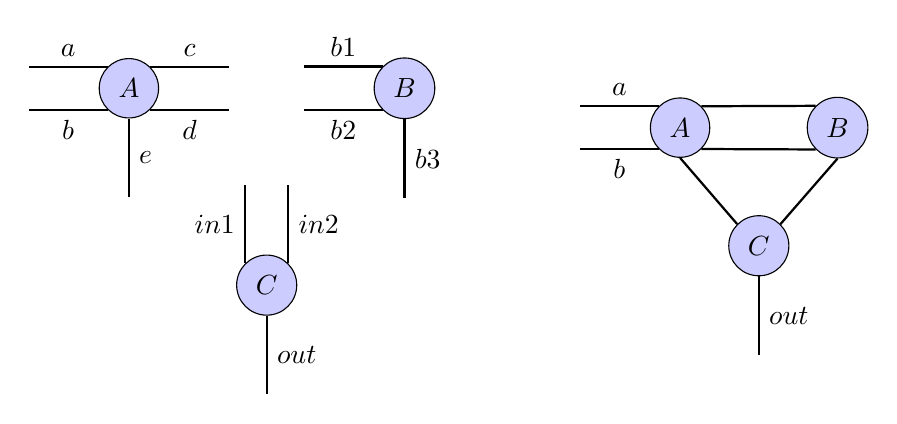
\begin{tikzpicture}

\node[det] (A) at (0,0) {$A$};
\draw[thick] (A.north east) -- node[above] {$c$} +(1,0);
\draw[thick] (A.south east) -- node[below] {$d$} +(1,0);
\draw[thick] (A.north west) -- node[above] {$a$} +(-1,0);
\draw[thick] (A.south west) -- node[below] {$b$} +(-1,0);
\draw[thick] (A.south) -- node[right] {$e$} +(0,-1);

\node[det] (B) at (3.5,0) {$B$};
\draw[thick] (B.north west) -- node[above] {$b1$} +(-1,0);
\draw[thick] (B.south west) -- node[below] {$b2$} +(-1,0);
\draw[thick] (B.south) -- node[right] {$b3$} +(0,-1);

\node[det] (C) at (1.75,-2.5) {$C$};
\draw[thick] (C.north west) -- node[left] {$in1$} +(0,1);
\draw[thick] (C.north east) -- node[right] {$in2$} +(0,1);
\draw[thick] (C.south) -- node[right] {$out$} +(0,-1);


\node[det] (Ap) at (7,-0.5) {$A$};
\node[det] (Bp) at (9,-0.5) {$B$};
\node[det] (Cp) at (8,-2) {$C$};

\draw[thick] (Ap.north east) -- (Bp.north west);
\draw[thick] (Ap.south east) -- (Bp.south west);
\draw[thick] (Ap.south) -- (Cp.north west);
\draw[thick] (Bp.south) -- (Cp.north east);

\draw[thick] (Ap.north west) -- node[above] {$a$} +(-1,0);
\draw[thick] (Ap.south west) -- node[below] {$b$} +(-1,0);
\draw[thick] (Cp.south) -- node[right] {$out$} +(0,-1);

\end{tikzpicture}

            \includegraphics[width=0.9\textwidth]{orus-images/fig4.pdf}
            \end{figure}}
        \end{column}
\end{columns}   


\end{frame}